\documentclass[11pt]{article}


%\documentclass[11 pt]{article}
\usepackage{graphicx}
\usepackage{float}

\usepackage[normalem]{ulem}

\usepackage[utf8]{inputenc}

\usepackage[square,sort,comma,numbers]{natbib}
\bibliographystyle{abbrvnat}
\setcitestyle{authoryear,open={(},close={)}} %Citation-related commands

\usepackage{setspace}

\usepackage{pdflscape}
%\doublespacing
\onehalfspacing
\usepackage[dvipsnames]{xcolor}
\usepackage{lineno}
\linenumbers
\usepackage{multicol}
\usepackage{hyperref}
\hypersetup{
	colorlinks=false,
%	linkcolor=blue,
%	filecolor=magenta,      
%	urlcolor=cyan,
	pdftitle={Overleaf Example},
	pdfpagemode=FullScreen,
}

\addtolength{\oddsidemargin}{-2.5cm}
\addtolength{\evensidemargin}{-1.5cm}

\addtolength{\textwidth}{5.5cm}

\addtolength{\topmargin}{-.875in}
\addtolength{\textheight}{1.75in}

% color can be used to apply background shading to table cells only
%\usepackage[table]{xcolor}

% array package and thick rules for tables
\usepackage{array}

% create "+" rule type for thick vertical lines
\newcolumntype{+}{!{\vrule width 2pt}}

% create \thickcline for thick horizontal lines of variable length
\newlength\savedwidth
\newcommand\thickcline[1]{%
  \noalign{\global\savedwidth\arrayrulewidth\global\arrayrulewidth 2pt}%
  \cline{#1}%
  \noalign{\vskip\arrayrulewidth}%
  \noalign{\global\arrayrulewidth\savedwidth}%
}

% \thickhline command for thick horizontal lines that span the table
\newcommand\thickhline{\noalign{\global\savedwidth\arrayrulewidth\global\arrayrulewidth 2pt}%
\hline
\noalign{\global\arrayrulewidth\savedwidth}}



%\author{Pending}


\begin{document}
%\title{Understanding the emergence of viral variants of concern via Bayesian molecular clock model selection}
\begin{flushright}

%\today
\end{flushright}
\begin{center}
	\begin{LARGE}
	\textbf{Supplementary results for: The phylodynamic threshold of measurably evolving populations}
	\end{LARGE}


Ariane Weber$^{1,*}$, Julia Kende$^{2}$, Sanni Översti$^{1, \ddagger}$ and Sebastian Duchene$^{3,4,\ddagger, *}$.
\end{center}

$^{1}$ Max Planck Institute of Geoanthropology, Jena, Germany.

$^{2}$ Institut Pasteur, Université Paris Cité, Bioinformatics and Biostatistics Hub, Paris, France.

$^{3}$ ED-ID unit, Dept of Computational Biology, Institut Pasteur, Paris, France.

$^{4}$ Peter Doherty Institute for Infection and Immunity, Dept of Microbiology and Immunology, University of Melbourne, Melbourne, Australia.
\newline

In fig. S\ref{figure:Fig1} we show the simulation results for a situation where the prior on the evolutionary rate is misleading and with most of its density falling on much higher values than those used to generate the data. Here, the prior on the evolutionary rate is $\Gamma(shape=1.5, rate=10^{4})$ (mean=$1.5\times 10^{-4}$, and 95\% range from $1.08 \times 10^{-5}$ to $4.7 \times 10^{-4}$), where as that for the population size is an exponential distribution with mean 5,000, and thus concentrated on the true value. Note that the resulting prior on the tree height is not misleading.

In fig. S\ref{figure:Fig2} we show the posterior distribution of the tree height for our empirical analyses of Hepatitis B virus with varying sampling window widths, while fig S\ref{figure:Fig3} shows the posterior distribution of the tree height for our empirical analyses with temporal sampling bias. The corresponding results with a misleading prior that favours low evolutionary rates and old divergence times are shown in figs \ref{figure:Fig4}, \ref{figure:Fig5}. The misleading prior on the evolutionary rate is $\Gamma(shape=1.5, rate=10^6)$, while for the population size it is an exponential distribution with mean 50,000.


Finally, figs \ref{figure:Fig6} and \ref{figure:Fig7} show the estimates of the evolutionary rate for these data using the `misleading' prior.

\begin{landscape}
	\begin{figure}[H]
		\begin{center}
			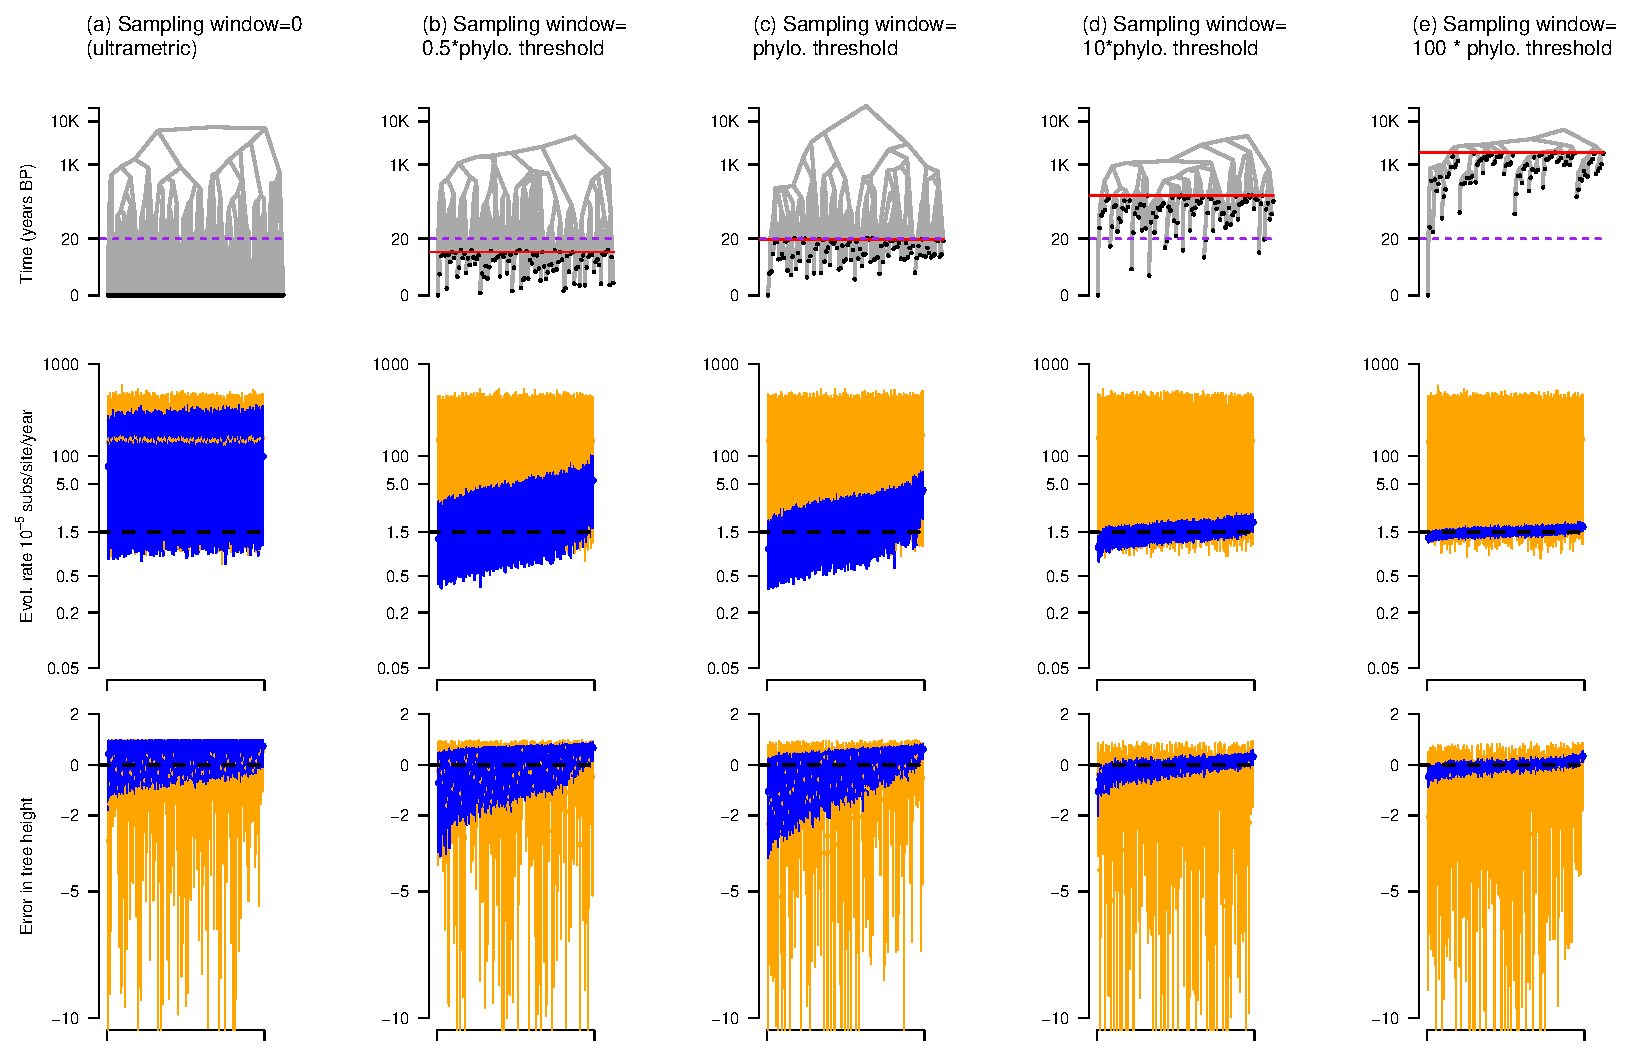
\includegraphics[scale=0.7, angle=0]{summary_all_estimates_misleading_upwards_prior.pdf}
			\caption{Simulations of varying sampling window widths with a `misleading prior'. Each column corresponds to a simulation setting: (a) is for ultrametric trees where all samples are collected at the same point in time, (b) is for the situation where the sampling window is 10 years (half the expected phylodynamic threshold), (c) is where the sampling window is exactly the expected phylodynamic threshold of 20 years. Scenarios (d) and (e) denote sampling windows that are 10 and 100 times the expected phylodynamic threshold. The first row is an example of a simulated phylogenetic tree with branch lengths scaled in units of time. The black circles represent genomic samples. The purple dashed line is the expected phylodynamic threshold and the solid red line is for the oldest sample, such that it represents the sampling window. Note that time here is shown in log$_{10}$ scale. The second row is the estimated evolutionary rate over 100 simulations. The dashed black line is the value used to generate the data (i.e. the ground truth), the dark blue bars are the posterior, and those in orange are the prior. For the prior and the posterior we use solid circles to show the mean estimate and the width of the error bars denotes the 95\% quantile range. The third row is the estimate of the error in tree height (the age of the tree). The error in tree height is calculated as $\frac{true-estimated}{true}$.}
			\label{figure:Fig1}
		\end{center}
		%		\centering
	\end{figure}
\end{landscape}

\begin{figure}[H]
    \begin{center}
        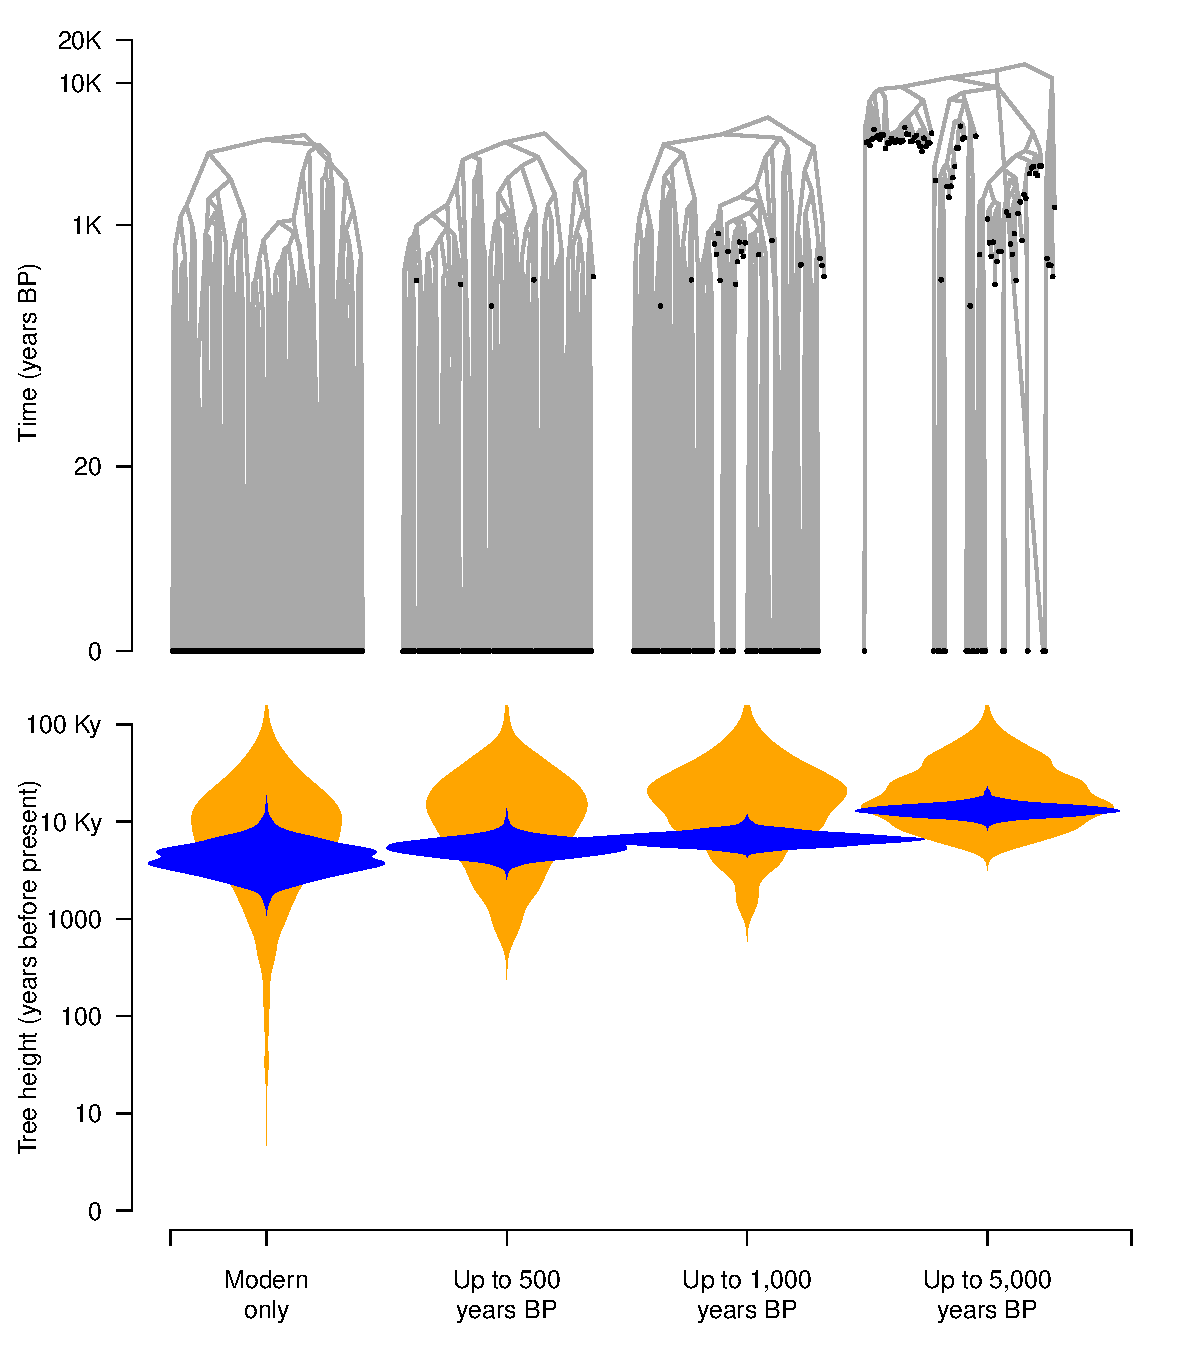
\includegraphics[scale=0.7, angle=0]{empirical_results_tree_height.pdf}
        \caption{Results from empirical analyses of Hepatitis B virus (HBV) ancient DNA data. The phylogenetic trees correspond to highest clade credibility trees from three analyses where the data were subsampled to include an increasing number of ancient samples. First, we consider a data set for which the samples are 95\% modern and the remaining 5\% being the most ancient. Then, we reduce the number of modern samples to 50\%, 25\% and 10\%, and the rest being ancient. Note that the sampling window is constant because we always retain the most ancient samples. In all cases the data sets consist of 100 genome samples. The violin plots show the posterior distribution of the tree height in blue and its corresponding prior in orange.}
        \label{figure:Fig2}
    \end{center}
    %		\centering
\end{figure}


\begin{figure}[H]
    \begin{center}
        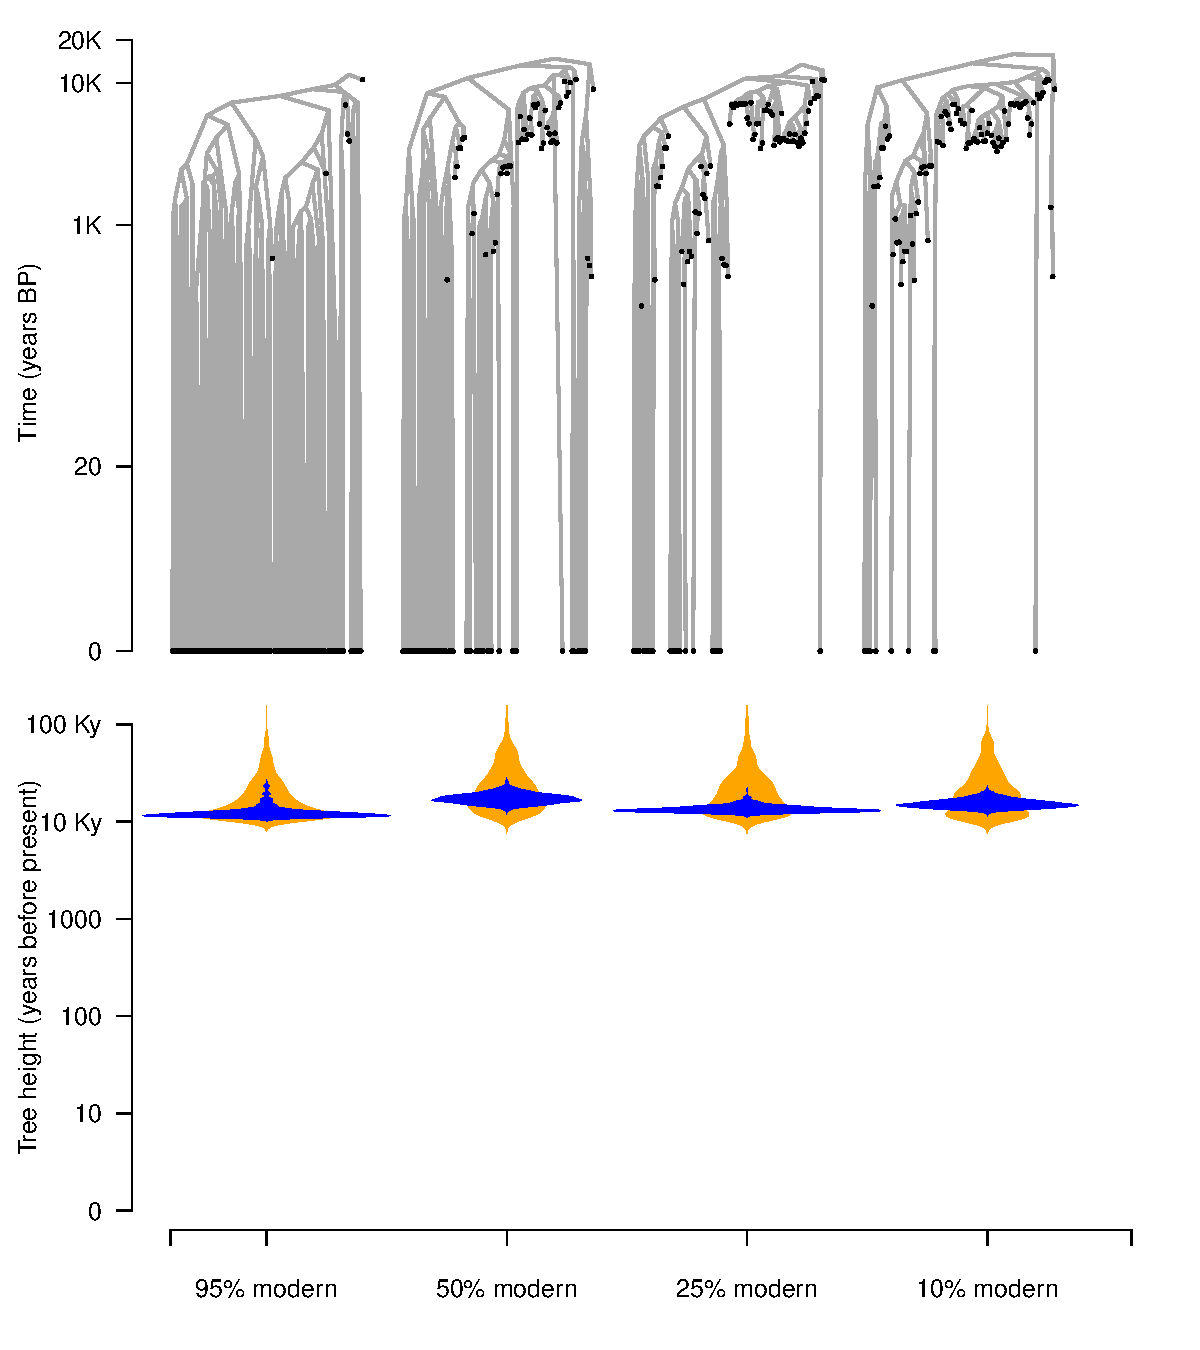
\includegraphics[scale=0.7, angle=0]{empirical_results_biased_root_height.pdf}
        \caption{Results from empirical analyses of Hepatitis B virus (HBV) ancient DNA data. The phylogenetic trees correspond to highest clade credibility trees from three analyses where the data were subsampled to include an increasing number of ancient samples. First, we consider a data set for which the samples are 95\% modern and the remaining 5\% being the most ancient. Then, we reduce the number of modern samples to 50\%, 25\% and 10\%, and the rest being ancient. Note that the sampling window is constant because we always retain the most ancient samples. In all cases the data sets consist of 100 genome samples. The violin plots show the posterior distribution of the tree height in blue and its corresponding prior in orange.}
        \label{figure:Fig7}
    \end{center}
    %		\centering
\end{figure}




\begin{figure}[H]
    \begin{center}
        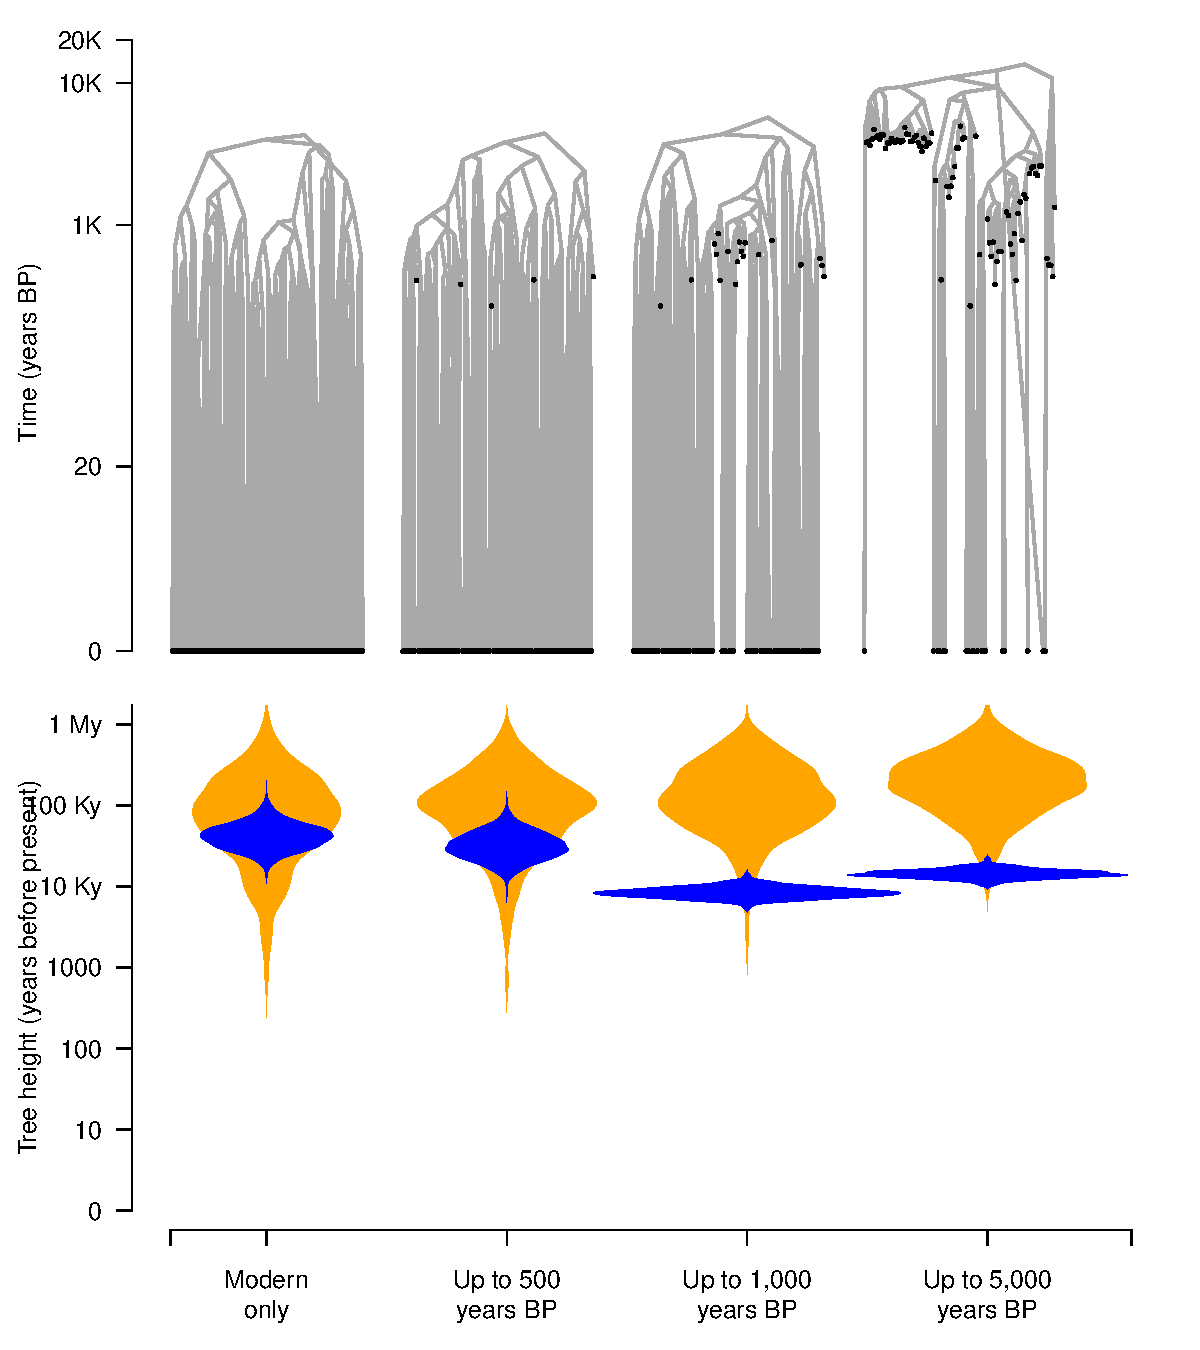
\includegraphics[scale=0.7, angle=0]{empirical_results_depth_misleading_prior_tree_height.pdf}
        \caption{Results from empirical analyses of Hepatitis B virus (HBV) ancient DNA data using a `misleading' prior configuration. The phylogenetic trees correspond to highest clade credibility trees from three analyses where the data were subsampled to include an increasing number of ancient samples. First, we consider a data set for which the samples are 95\% modern and the remaining 5\% being the most ancient. Then, we reduce the number of modern samples to 50\%, 25\% and 10\%, and the rest being ancient. Note that the sampling window is constant because we always retain the most ancient samples. In all cases the data sets consist of 100 genome samples. The violin plots show the posterior distribution of the tree height in blue and its corresponding prior in orange.}
        \label{figure:Fig3}
    \end{center}
    %		\centering
\end{figure}






\begin{figure}[H]
    \begin{center}
        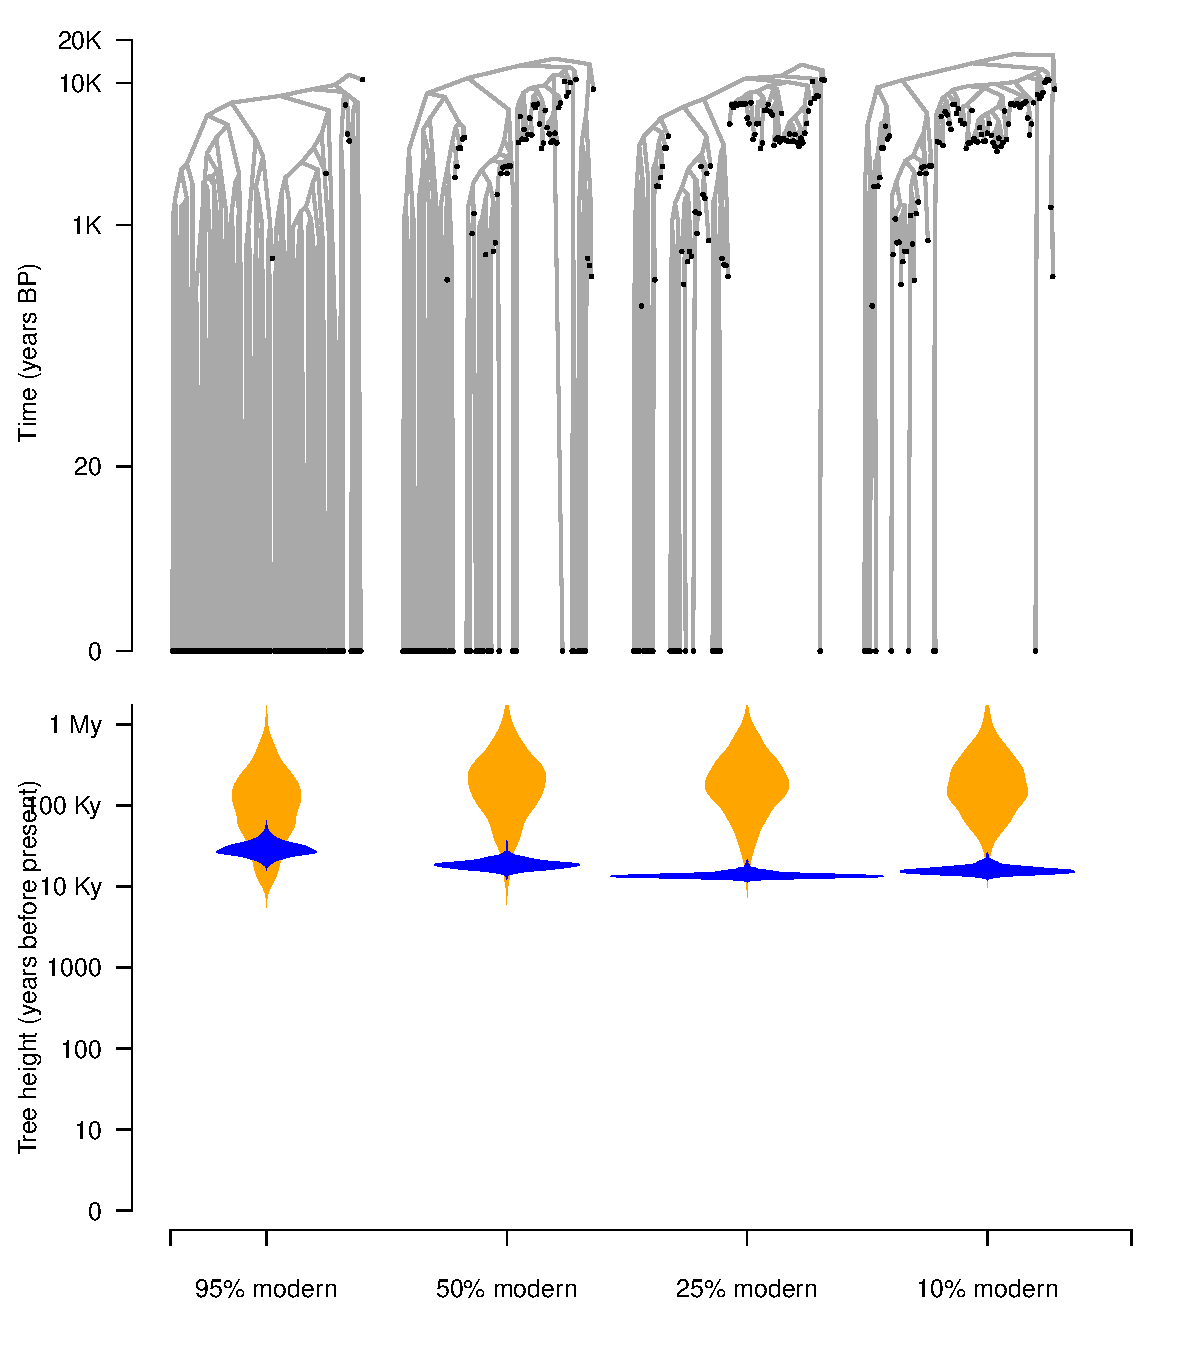
\includegraphics[scale=0.7, angle=0]{empirical_results_biased_misleading_prior_root_height.pdf}
        \caption{Results from empirical analyses of Hepatitis B virus (HBV) ancient DNA data using a `misleading' prior. The phylogenetic trees correspond to highest clade credibility trees from three analyses where the data were subsampled to include an increasing number of ancient samples. First, we consider a data set for which the samples are 95\% modern and the remaining 5\% being the most ancient. Then, we reduce the number of modern samples to 50\%, 25\% and 10\%, and the rest being ancient. Note that the sampling window is constant because we always retain the most ancient samples. In all cases the data sets consist of 100 genome samples. The violin plots show the posterior distribution of the tree height in blue and its corresponding prior in orange.}
        \label{figure:Fig5}
    \end{center}
    %		\centering
\end{figure}


\begin{figure}[H]
    \begin{center}
        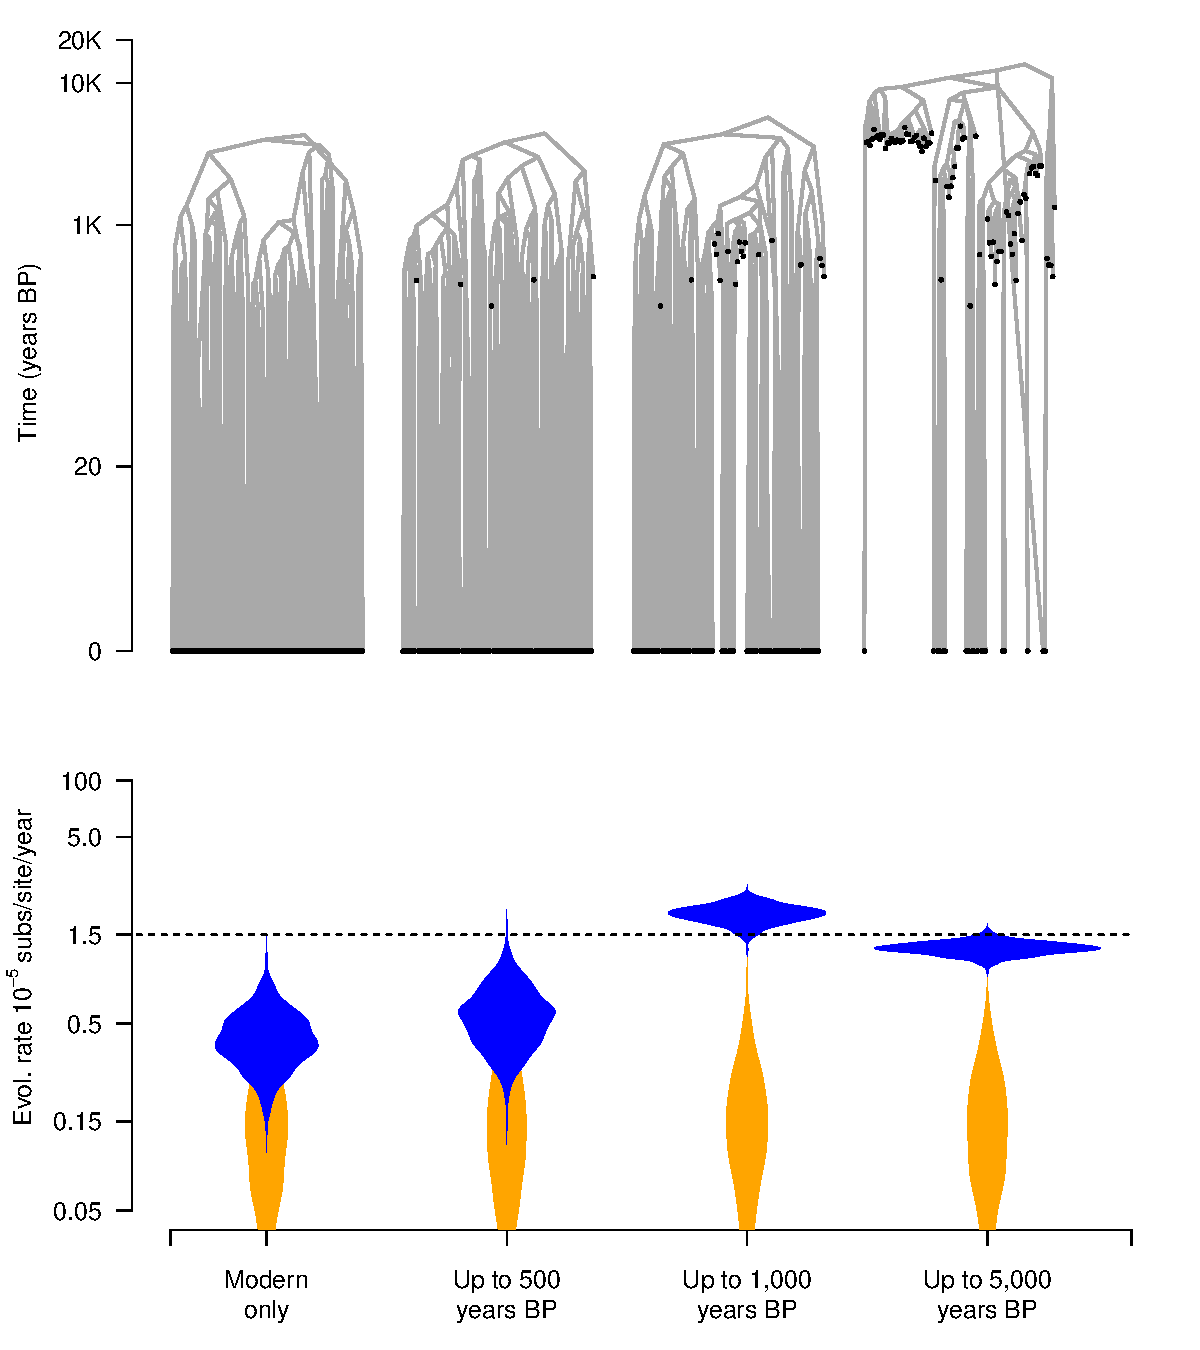
\includegraphics[scale=0.7, angle=0]{empirical_results_depth_misleading_prior.pdf}
        \caption{Results from empirical analyses of Hepatitis B virus (HBV) ancient DNA data under a `misleading' prior configuration. The phylogenetic trees correspond to highest clade credibility trees from three analyses where the data were subsampled to include an increasing number of ancient samples. First, we consider a data set for which the samples are 95\% modern and the remaining 5\% being the most ancient. Then, we reduce the number of modern samples to 50\%, 25\% and 10\%, and the rest being ancient. Note that the sampling window is constant because we always retain the most ancient samples. In all cases the data sets consist of 100 genome samples. The violin plots show the posterior distribution of the evolutionary rate in blue and its corresponding prior in orange.}
        \label{figure:Fig6}
    \end{center}
    %		\centering
\end{figure}



\begin{figure}[H]
    \begin{center}
        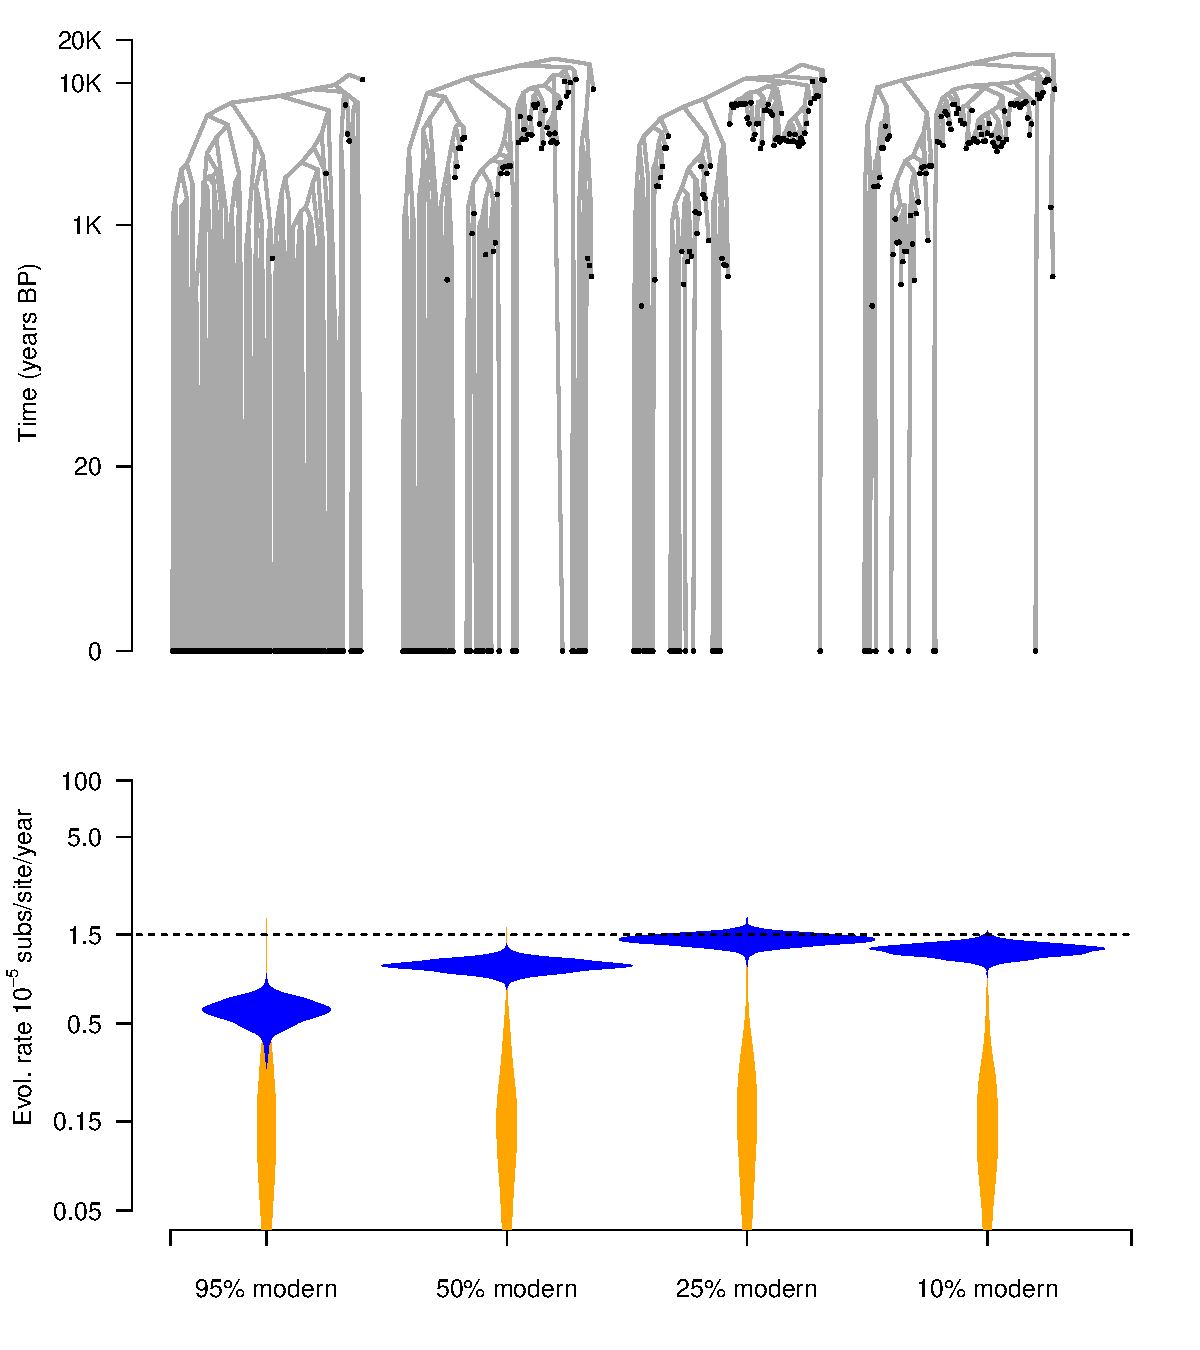
\includegraphics[scale=0.7, angle=0]{empirical_results_biased_misleading_prior.pdf}
        \caption{Results from empirical analyses of Hepatitis B virus (HBV) ancient DNA data using a `misleading' prior. The phylogenetic trees correspond to highest clade credibility trees from three analyses where the data were subsampled to include an increasing number of ancient samples. First, we consider a data set for which the samples are 95\% modern and the remaining 5\% being the most ancient. Then, we reduce the number of modern samples to 50\%, 25\% and 10\%, and the rest being ancient. Note that the sampling window is constant because we always retain the most ancient samples. In all cases the data sets consist of 100 genome samples. The violin plots show the posterior distribution of the evolutionary rate in blue and its corresponding prior in orange.}
        \label{figure:Fig7}
    \end{center}
    %		\centering
\end{figure}


\end{document}